\section{Episode 31: NOTICE ME SENPAI!!!}

\begin{multicols}{2}

\DndDropCapLine{D}ear Diary.\medskip

Well here we are in the tower (but it’s underground so i still think it’s just a long cellar) of Mr Rubriks. We stood looking at a blood scrawled message on the wall. I flicked up Pilch’s helmet and read “Beware, do not enter. The great devourer lies within”. It didn’t sound like the best thing. Jeremy threw a spear at the lovely mauve forcefield. It just rebounded but he caught it in a cool way. Riphard looked upset about the fact he didn’t die. Riphard decided he wanted to kill Stanri for literally no reason.\medskip

Kolo decided to step up and take the lead by becoming red and going to the door that was not the forcefield. He walked straight back out his unhappy face on. Turns out there were snakes behind there. Or snake men. One opened the door and peeked through. They told us to freeze. The snakey men looked shocked that we understood them and pointed out that they had not seen any soft skins for a long time. Kolo told them we just wanted to be friends. Myron was alarmed and got ready to fire at them but Kolo made him back down. Kolo told them we were inspectors and luckily they didn’t ask about what. They looked at Jeremy with hungry eyes. Riphard farted and inadvertently told the snake people that he wanted to fist both their mother’s snake anuses simultaneously with both arms. Kolo defused the situation. We took a moment to appreciate the forms of the snakey men. They were basically backwards-mermaid-snakes. That was the best way to describe them.\medskip

We followed them through the door and tried to do our best to look like we were inspecting things. The snakey men seemed to change colours a little bit as they walked through the doors. Kolo pointed out a nice statue to steal which I was originally excited about but then I as I got closer I realised it was big. Riphard tried to walk through a door but couldn’t. Kolo asked them to open the door and wanted their names and numbers. It turns out they are “Sssidney” and “Sssssecil”. WE met some other snakey people and they had a little conversation. Turns out we’re going to see the Queen. They told their friends that we were inspectors. The ruse was working perfectly. I was curious if they layed eggs. Kolo asked but it turned out to be too personal. They talked about how they were slaves. It sounded like they needed emancipation is. Myron politely pointed out that perhaps now wasn’t precisely the right time for emancipation.\medskip

We followed Sssidney and Sssssecil into the throne room. Stanri stayed in the doorway to keep it open and Myron looked around the room with his dark, intense eyes, surveying the room in all his wisdom. One of the snake people had a lovely long robe and it was clear she was the snake queen. She wanted to know who we were and Sssidney introduced us. She addressed us directly. Kolo admitted we were the trade and civil disputes inspectors. She wanted to know where we came from, but she didn’t seem to know what Velterra was. It was a little confusing. Kolo nominated Myron as our diplomat. He complimented her house and asked if she was planning on stopping us. It seemed a little direct and she pointed out that no-one that went downstairs returned. She seemed happy that we voluntarily wanted to go downstairs and it would save them a job of making an offering to the great devourer. She seemed adamant that if we went downstairs we wouldn’t have any more work to do. Myron asked a lot about treasure but they didn’t seem to have any concept of what that would be. The queen said she thought her egg producing days were soon to come to an end I KNEW THEY LAID EGGS. The queen started telling us about their old friend Sssseinfeld who was a funny snake. The funny joke was “how many snakes does it take to sate the great devourers”. Probably just one as he got eaten. There are five great devourers apparently. Each takes different forms and stalks the lower levels and devours things which makes sense and also there used to be more but they got devoured. Myron asked the snakey people what they eat and they said that they farm monkeys. What do the monkeys eat is the next logical question and the answer is poop. The perfect food chain. Riphard asked the queen for extra people to help but she couldn’t spare the snakeys. He was horrified that they didn’t want to help and just sacrifice their unborn children. Riphard tried to kick the door open and almost succeeded but almost does not mean the same as did. A rattley snake man opened the door for him with his rattle. Kolo and Jeremy had a little rest.\medskip

Myron asked me to make him a minecart. I was a little confused but it must have been important. Kolo and Jeremy went out into a garden through a door. It was sad that they didn’t know that this was here because if they did maybe they wouldn’t have to eat so many poop monkeys. I managed to lay about 8 ft of rail but then there wasn’t enough time and I was trying to work really fast to impress Myron but then he said that he wasn’t impressed and that I should have made the cart first and of course he’s right because what is even the point of a railroad without any carts and I felt horrible about myself and also fat. I followed everyone into the garden and tried not to let Myron see me crying.\medskip

Vudong jumped off the stairs monkey style. Riphard tried to slide down the bannister but there wasn’t one so he didn’t. The rest of us took the stairs. As we walked down we heard a large screeching sound! A creature jumped out of the treetops and it was like a bird and had tentacles coming out of its back and had a beak and more tentacles. I tried to shoot it through the trees but my eyes were still all leaky so I missed like the useless gabrin I am. The tentacle bird went for Riphard straight away and hit him with both legs and then grabbed him in its talons and then it flew him away. Kolo tried to hit it but the trees were too dense. Time seemed to stand still for too long and then Jeremy suddenly did the biggest jump I ever really saw and went up in the trees and then to the wall and then incredibly he jumped at the tentacle bird! It was amazing. He hit it with both staffs and then they all fell to the floor! Jeremy floated to the ground but the birdy still had Riphard all grabbed up. Myron couldn’t hit it and Riphard did his magic fire thing. I still couldn’t hit it because it was all on the floor. It tried to hit Riphard again but it looked to stunned. Riphard tried to get out of its claws but he was too weak. Jeremy fortunately knew what was going on and he jumped over like a brave little monkey and just started beating the birdy. Myron took a shot and a chunk of blood and feathers and severed tentacles flew off it. Riphard tried to shoot it but couldn’t quite hit. Kolo took aim and shot the birdy with his poisony arrow. Didn’t even matter because it died just like that. As he was disembowelling we found out it was terrible. The whole digestive system was backwards so it had a botbot for a mouth. Kolo started inspecting and I asked him why because I thought it was a trick but then he reminded me that we were inspectors and I had completely forgotten. I didn’t want him to think I was slacking so I started writing hard but I was really just drawing a little picture of what I thought a nice dress would like like for Jeremey. Kolo offered Riphard a KokaKola™ and he took it. Riphard got a fever. He seemed to like the KokaKola™. He started REALLY touching himself. I had to look away.\medskip

Jeremy crouched down and stealthily and headed northwards. We followed him and found a yellow doorway. Myron turned himself purple and headed through the door. Kolo followed. As they went in they saw a teleportation circle all covered in blood and then suddenly there was a bang and a big floppy meaty monster fell into the room. I quickly followed in and shot it hard in the meaty face. Kolo followed up quickly with his own shot, the old gabrin 2-2. I thought he might run out and hide back through the door but he looked at me and I knew he knew the gabrins should always be close together, fighting the good fight. Myron went up straight to it and hit it with his funny gun. Jeremy followed up with all his flailing monkey madness and he even kicked it in the naughty place. Riphard shot it. I shot it. Kolo shot it. Myron shot it (and stabbed it). Jeremy hit it (lots). Suddenly the creature started flashing all purple and everything really hurt in my brain. Riphard tried to shoot it but missed and then I did too. The brain pain was too much. It was like all the worst, most painful memories of multiple creatures all rushed through me all at once. Myron took out his glove that he got and punched the meaty monster in the face. There wasn’t so much face of it left after that. Not much at all, just a frothing hole. Kolo was impressed but I wasn’t in the mood to be impressed with Myron right now. Delilah showed up and mentioned how terrible men are and I agreed then got busy doing my inspections. The place used to be a teleportation circle but it’s magic programming seems to have got degraded overtime. I advised everyone to walk around the circle.\medskip

After a short little rest we decided to go on. Kolo took the lead and said he found an office full of diaries and books and things. One was from an apprentice of Rubriks and his diary said that he was not so keen on being an employee anymore because all the magic was drying up. Kolo found some shiny trinkets and handed them to me too. Kolo gave me some nice advice and I gave him a hug to say thank you. Kolo saw a statue and made a mental note to complement his imaginary notes that he was taking because he was worried he might forget the latter and did not want to forget. We found a door that had no colour and it had two odd statues next to it that had their hands all out. Kolo and Myron had a look but couldn’t find any lasers so we sent the monkey in just to be safe. He tried touching it with his spears but nothing happened so he tried to throw a little monkey at the door. He threw it really hard and the little monkey was basically just flat afterwards. Myron got annoyed and tried to grab the monkey to throw him at the door but Jeremy escaped. Kolo went to take another look at the door so he made himself blue. Myron looked stupid but also very short in a confident way. Kolo remembered that the statue before had stone vials of different colours in each hand. He tried to put some of the colours on the statues that had outstretched palms. Nothing happened. He swapped them over. Again it didn’t work. Jeremy suggested red and blue and the door opened. I gave him a friendly pat as if to say “well done. You got there in the end”. There was another weird fused creature on the other side of the door. I imagined this one would be a breeze too. I feel a lot like the snakey people were getting a bit carried away when they described the threat level here.\medskip

We got ready to fight (except for Delilah who was in a mood with Riphard still). Kolo led the way blazing all the arrows out of his quiver and into the bow and into the tripleman. Riphard seemed to recognise the tripleman and kept shouting the “alansugar”. Myron screamed “cronenborg”. I missed and the Myron ran in and yelled “I’m fired” and laughed to himself and pummeled the thing. Jeremey went all out and I could not even make out what was going on all his monkey arms and legs were moving so fast indeed. Riphard filled us with a brave defensive fire, shot it, and then ran away to hide shouting “It’s up to you guys”. Kolo pulled his bow extra hard and shot it in the middle head and it did not look good. I shot it again for good measure. Myron unloaded a shot into its abdomen area, as it brought its arms down Myron hoisted himself up then put his gun in its throat and shot into its horrific monstrous body. So cool. I’m so confused. Jeremy jumped up and started hitting it again. Riphard shot it. Kolo did. And then I blew it to pieces. Immiviseceration to the maximum. We all took a moment to talk about how disappointed we were in these devourers and how poorly we collectively thought about the snakey people.\medskip

We carried on into the next room, and found a stove. Kolo seemed very interested in it. I pointed out that it didn’t have a safety sticker and Kolo seemed enthused. He spent some time fashioning a small condemnation sign. I’ve always admired my brother’s dedication to health and safety protocol. When he was a very young gabrin he won the school nomination for most likely to be a health and safety inspector. Oh how he would spend those long evenings in gabrin land writing risk assessments and HAZOPs. Myron went investigating all the doors. He seemed to be on it and was doing like this crazy backwards walk where it looked like he was going forwards but he was going backwards. Inefficient but thrilling all the same. He had found some diary pages that Kolo translated: “It’s been 20 years since Rubriks sealed himself away. The magic has begun to wane. My power is not once it once was. I fear that this tower may become untenable in the future. Should I keep studying and hope magic returns and leave or make my own way in the world”. Kolo explained the words to Myron and also that the gabrin’s are related. He accepts this and admits he didn’t want to assume for fear of being racist. Jeremy kept trying to meditate. Kolo tried to kick him but he was too oily from the dangerous cooker. Stanri tried to gud Jeremy but they were both too oily. Cute and sad at the same time.\medskip

\textbf{Epilogue}\medskip

Alan looked over at the strange man in front of him. The impression he got was not good but dear god he needed this job. He didn’t know how he was going to look Melania and the girls in the face if he failed again. The old man stared at him with his shrill eyes. “I notice here on your CV it says you are good at working closely with other people?”, he said in his voice that sounded both mad and dull at the same time. The man was most likely a closet homsexual Alan thought to himself, at once chiding himself for his internal bigotry. ‘It’s 6342 man for Sin’s sake. Not the dark ages. Live and let live’ he corrected himself. “Yes I have worked in many teams and have good … team skills”, he said earnestly. The old man nodded in approval. The nod seemed to come not only from his head but his knees as well. Alan didn’t even understand how that could be. The old man looked at him intensely and said “hypothetical scenario, you are interviewed for a standard managerial job in an underground tower in which you have had to travel to by means of a magical transportation circle, and the man interviewing you is quite mad and intends to offer you a job under false pretences and once you have accepted he will magically sedate you and create a monstrous hybrid human creation by robbing you of your humanity through psychic devastation then sewing you to two other unwilling participants. You will then live for hundreds of years and fight against any intruders into the afroementioned tower and also become elevated to the status of vengeful gods that must be constantly appeased by offerings of snake eggs and monkeys reared on snake faeces”. The man paused. “What do you think are your relevant skills for this position?”. Alan took a deep breath. One of these ‘crazy interview questions’ designed to test your problem solving skills. He’d read a whole book on this and done that day course using the last of the babie’s milk money. He knew that it hadn’t been squandered. Alan smiled. “Well, as I say, I enjoy working closely with people….”\medskip

https://youtu.be/vNuVifA7DSU?t=59

\end{multicols}

\vspace*{5mm}

\begin{center}
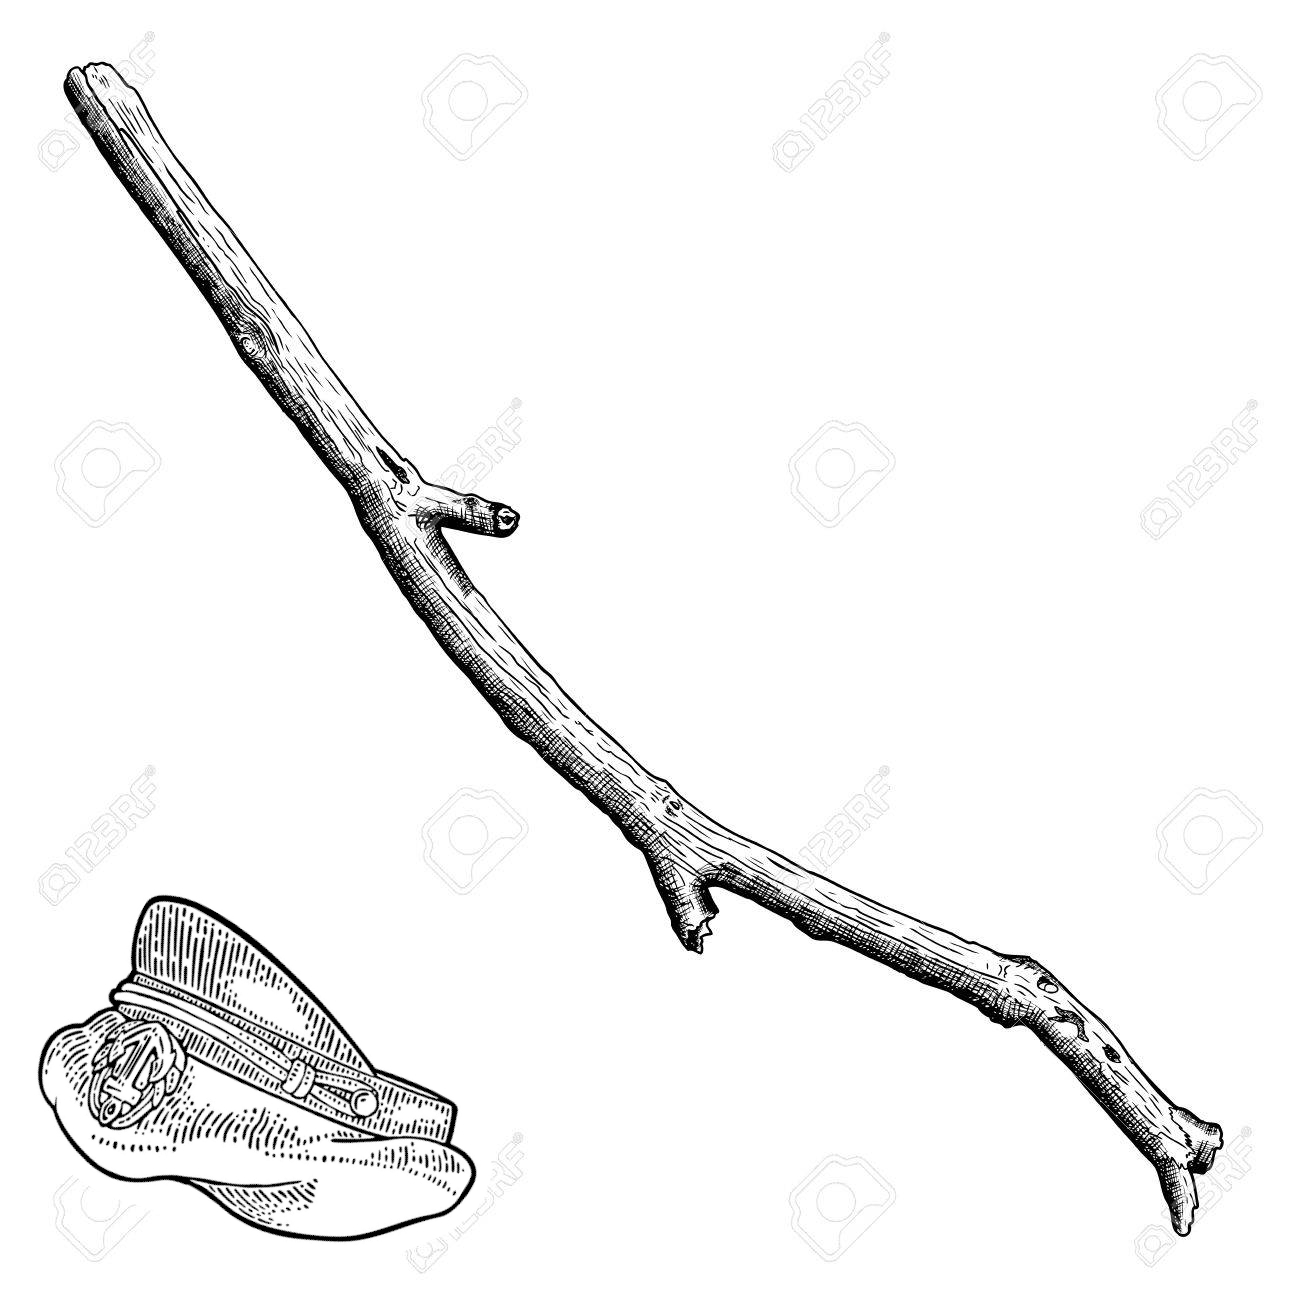
\includegraphics[width=\textwidth]{./content/img/xxx.jpg}
\begin{figure}[h]
\end{figure}
\end{center}

\clearpage